% ##QuantumErrorCorrection ##Decoding ##SurfaceCode ##CorrelatedErrors 
\documentclass[a4paper, english]{scrartcl}
\usepackage[utf8]{inputenc}
\usepackage{amsmath}
\usepackage{amsfonts}
\usepackage{amssymb}
\usepackage{babel}
\usepackage[cm]{fullpage}
\usepackage{float}
\usepackage{graphicx}
\usepackage{helvet}
\usepackage{hyperref}
\usepackage{mathtools}
\usepackage{nicefrac}
\usepackage{tikz}
\usepackage{pgfplots}
\usepackage{placeins}
\usepackage{verbatim}
\usepackage{xcolor}
\definecolor{gr}{gray}{0.9}
\renewcommand{\familydefault}{\sfdefault}
\title{Quantum Error Correction}
\subtitle{Correlated Decoding as Bilinear Programming}
\author{Ben Criger}
\date{\today}
\input{Qcircuit.tex}
\usepackage{amsmath}
\usepackage{bbold}
\usepackage{color}
\usepackage{stmaryrd}
\usepackage{calc}
\usepackage{verbatim}
\usepackage{mathtools}
\usepackage{xspace}
\DeclarePairedDelimiter{\ceil}{\lceil}{\rceil}
\DeclarePairedDelimiter{\floor}{\lfloor}{\rfloor}
\DeclareMathOperator{\Span}{span}
\usepackage{tikz}
\usetikzlibrary{calc}
\providecommand{\polygon}[2]{%
  let \n{len} = {2*#2*tan(360/(2*#1))} in
 ++(0,-#2) ++(\n{len}/2,0) \foreach \x in {1,...,#1} { -- ++(\x*360/#1:\n{len})}}

\DeclareMathOperator\erf{erf}
\DeclareMathOperator\erfc{erfc}

\newsavebox\CBox
\newcommand\hcancel[2][0.5pt]{%
  \ifmmode\sbox\CBox{$#2$}\else\sbox\CBox{#2}\fi%
  \makebox[0pt][l]{\usebox\CBox}%  
  \rule[0.5\ht\CBox-#1/2]{\wd\CBox}{#1}}

\providecommand{\drv}[1]{\frac{\partial }{\partial #1}}
\providecommand{\drf}[2]{\frac{\partial #1}{\partial #2}}
\providecommand{\ddrf}[3]{\frac{\partial^2 #1}{\partial #2 \partial #3}}
\providecommand{\ddid}[3]{\frac{\partial^2 #1}{\partial #2 \partial #3} = \dfrac{\partial^2 #1}{\partial #3 \partial #2}}

\providecommand{\tr}{\mathrm{tr}}
 
\providecommand{\ket}[1]{\left \vert #1 \right \rangle}
\providecommand{\bra}[1]{\left \langle #1 \right \vert}
\providecommand{\braket}[2]{\left \langle #1 \left \vert #2 \right. \right \rangle}
\providecommand{\angles}[1]{\left \langle #1 \right \rangle}
\providecommand{\elem}[3]{\left \langle #1 \left \vert \vphantom{#1#2#3} #2 \right \vert #3 \right \rangle}
\providecommand{\delem}[2]{\left \langle #1 \left \vert \vphantom{#1#2} #2 \right \vert #1 \right \rangle}
\providecommand{\ketbra}[2]{\ket{#1} \! \bra{#2}}
\providecommand{\proj}[1]{\ketbra{#1}{#1}}
\providecommand{\twonorm}[1]{\| #1 \|_2}
\providecommand{\abs}[1]{\left \vert #1 \right \vert}
\providecommand{\set}[1]{\left \lbrace #1 \right \rbrace}
\providecommand{\group}[1]{\left \langle #1 \right \rangle}
\providecommand{\red}[1]{\textcolor[rgb]{0.5,0,0}{#1}}
\providecommand{\blue}[1]{\textcolor[rgb]{0,0,0.5}{#1}}
\providecommand{\green}[1]{\textcolor[rgb]{0,0.5,0}{#1}}
\providecommand{\conjecture}[1]{\red{#1 (check this).}}
\providecommand{\future}[1]{\green{#1 (do this later).}}
\providecommand{\id}{\hat{\mathbb{1}}}
\providecommand{\com}[2]{\left[#1,\,#2 \right]}
\providecommand{\acom}[2]{\left \lbrace #1,\,#2 \right \rbrace}
\providecommand{\diss}[2]{\mathcal{D}\left[ #1 \right]\left( #2 \right)}
\providecommand{\meas}[2]{\mathcal{M}\left[ #1 \right]\left( #2 \right)}
\providecommand{\lindtwo}[2]{ #1 #2 #1^{\dagger} - \dfrac{1}{2} \left \lbrace #1^{\dagger} #1,\,#2 \right \rbrace }
\providecommand{\lindthree}[3]{ #1 #2 #3 - \dfrac{1}{2} \acom{#3 #1}{#2} }
\providecommand{\lindfour}[4]{ #1 #2 #3 - \dfrac{1}{2} \acom{#4}{#2} }
\providecommand{\meastwo}[2]{ #1 #2 + #2 #1^{\dagger} - \tr \left( #1 #2 + #2 #1^{\dagger} \right) #2 }
\providecommand{\tenscom}[4]{\com{#1\otimes #2}{#3 \otimes #4}=\dfrac{1}{2}\left( \com{#1}{#3} \otimes \acom{#2}{#4} + \acom{#1}{#3} \otimes \com{#2}{#4} \right)}
\providecommand{\tenscomsimple}[4]{\com{#1\otimes #2}{#3 \otimes #4} = #1 #3 \otimes \com{#2}{#4} + \com{#1}{#3} \otimes  #4 #2}
\providecommand{\tensacom}[4]{\acom{#1\otimes #2}{#3 \otimes #4}=\dfrac{1}{2}\left( \com{#1}{#3} \otimes \com{#2}{#4} + \acom{#1}{#3} \otimes \acom{#2}{#4} \right)}
\providecommand{\trace}[1]{\mathrm{tr} \left( #1 \right)}
\providecommand{\comp}{\mathop{\bigcirc}}
\providecommand{\swap}{\textsc{swap}\xspace}
\providecommand{\cnot}{\textsc{cnot}\xspace}
\providecommand{\cz}{\textsc{cz}\xspace}
\providecommand{\col}{\textrm{col}}
\providecommand{\qec}[3]{\llbracket #1,\,#2,\,#3 \rrbracket}
\providecommand{\set}[1]{\left \lbrace #1 \right \rbrace}
\renewcommand{\Im}{\textrm{Im}}
\renewcommand{\Re}{\textrm{Re}}
\providecommand{\lind}{\mathcal{L}}
%\providecommand{\norm}[2]{\left \vert \left \vert #2 \right \vert \right \vert_{#1}}
\providecommand{\supp}[1]{\mathrm{supp}\left( #1 \right)}
\providecommand{\given}{\, \middle \vert \,}
\providecommand{\suchthat}{\, \middle \vert \,}
\providecommand{\diag}[1]{\mathrm{diag}\left( #1 \right)}
\providecommand{\ct}{^{\dagger}}

\providecommand{\norm}[1]{\left \Vert #1 \right \Vert} %only works with amsmath

\providecommand{\ncrit}{$n_{\textrm{crit}}$\xspace}

\renewcommand{\th}{\textrm{th}}
\newcommand{\prob}[1]{p\left(#1 \right)}
\newcommand{\cprob}[2]{p\left(#1\,\left\vert\vphantom{#1#2}\right. #2\right)}

\makeatletter
\providecommand{\pr}[2]{p\left(#1\,\middle|\,#2\right)}
\newcommand{\pushright}[1]{\ifmeasuring@#1\else\omit\hfill$\displaystyle#1$\fi\ignorespaces}
\newcommand{\pushleft}[1]{\ifmeasuring@#1\else\omit$\displaystyle#1$\hfill\fi\ignorespaces}
\makeatother
\newlength\figureheight
\newlength\figurewidth
\setlength\figureheight{7cm}
\setlength\figurewidth{12cm}

\providecommand{\cnot}{\textsc{cnot}}

\usetikzlibrary{decorations.pathreplacing, decorations.pathmorphing, shapes.geometric, calc}

\begin{document}
\maketitle
\section{Introduction}
The toric code is a popular 2D nearest-neighbour LDPC code whose decoding can be efficiently accomplished by minimum-weight perfect matching. 
Qubits are placed on the edges of a square tiling of a 2D torus, and are subjected to one of three errors, with labels $X$, $Y$ and $Z$:
\begin{figure}[!h]
\centering
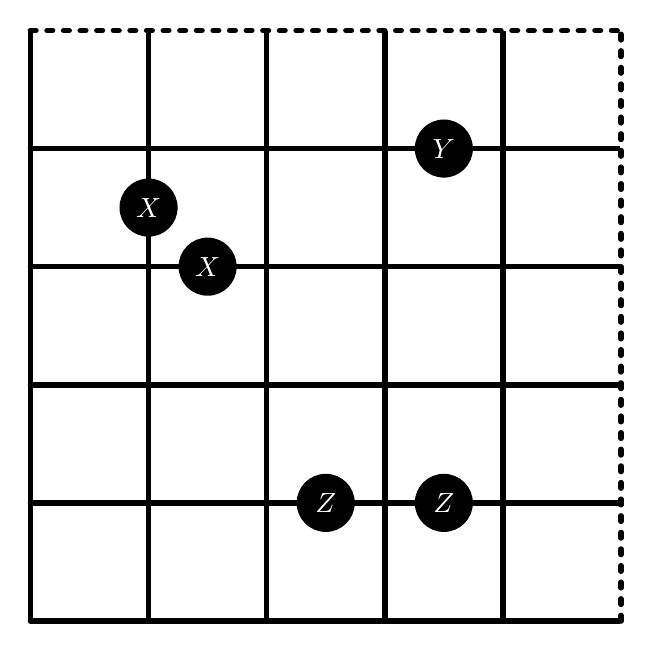
\begin{tikzpicture}[scale=0.75]
\draw[step=2, line width = 2pt, loosely dotted, line cap=round, line join=round] (0,0) grid (10,10);
\draw[step=2, line width = 2pt] (0,0) grid (9.99,9.99);
\foreach \x/\y/\err in {5/2/$Z$, 7/2/$Z$, 3/6/$X$, 2/7/$X$, 7/8/$Y$}{
\fill[black] (\x,\y) circle(14pt);
\node[white] at (\x,\y){\err};
}
\end{tikzpicture}
\caption{5-by-5 toric code lattice with an error configuration.
Qubits are supported on each edge, of which there are 50.
Five of these qubits have been subject to an error, drawn from the set $\set{X,\,Y,\,Z}$. 
Edges with no marker are not subject to error. 
Dotted edges indicate `wrapping around' the boundary to create a torus.}
\end{figure}

The parity checks of this code respond to $X$ and $Z$ errors, indicating when an odd number of $X$ errors surround a tile, and an odd number of $Z$ errors surround a vertex:
\begin{figure}[!h]
\centering
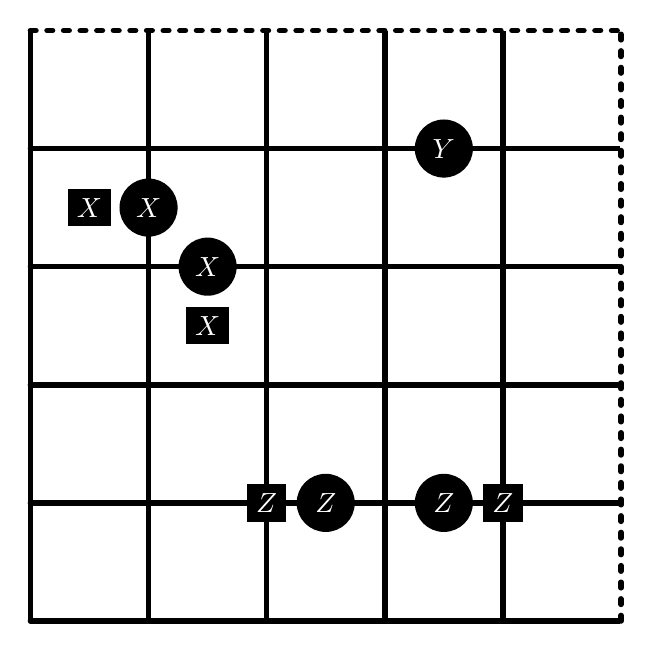
\begin{tikzpicture}[scale=0.75]
\draw[step=2, line width = 2pt, loosely dotted, line cap=round, line join=round] (0,0) grid (10,10);
\draw[step=2, line width = 2pt] (0,0) grid (9.99,9.99);
\foreach \x/\y/\err in {5/2/$Z$, 7/2/$Z$, 3/6/$X$, 2/7/$X$, 7/8/$Y$}{
\fill[black] (\x,\y) circle(14pt);
\node[white] at (\x,\y){\err};
}
\foreach \x/\y/\synd in {4/2/$Z$, 8/2/$Z$, 3/5/$X$, 1/7/$X$}{
\node[fill=black] at (\x,\y){\textcolor{white}{\synd}};
}
\end{tikzpicture}
\caption{Syndromes corresponding to $X$ and $Z$ errors.}
\end{figure}
\FloatBarrier
One thing to notice about these syndromes is that, if a continuous chain of errors of the either $X$ or $Z$ type appears on the lattice, two syndromes will appear at the endpoints of the chain.
If only $X$ and $Z$ errors occur, then, the assignment of an error to a given syndrome in the toric code can be reduced to minimum-weight perfect matching, since the probability of an error chain can be expressed as a function of the distance between the syndromes.

If $Y$ errors could be independently detected and decoded in the same fashion, we'd be done. 
The problem is that, due to Quantum Code Technicalities\textsuperscript{\textregistered}, a $Y$ error produces a pair of $X$ \emph{and} $Z$ syndromes:
\begin{figure}[!h]
\centering
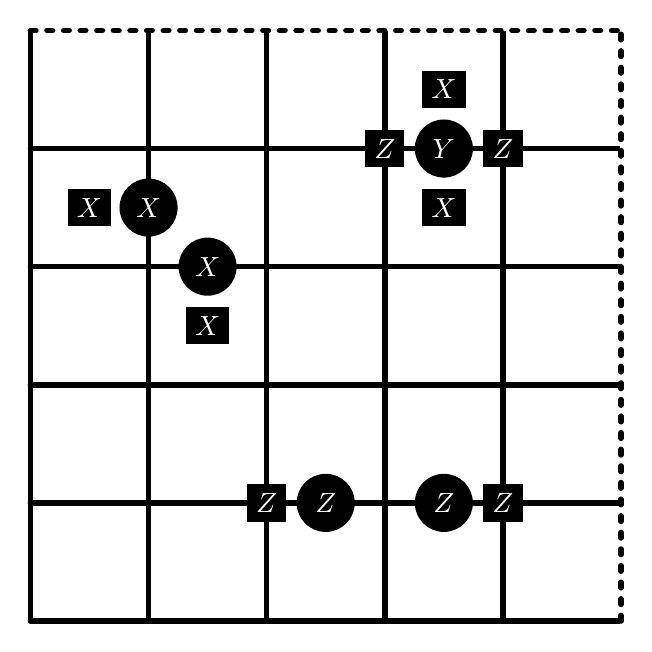
\begin{tikzpicture}[scale=0.75]
\draw[step=2, line width = 2pt, loosely dotted, line cap=round, line join=round] (0,0) grid (10,10);
\draw[step=2, line width = 2pt] (0,0) grid (9.99,9.99);
\foreach \x/\y/\err in {5/2/$Z$, 7/2/$Z$, 3/6/$X$, 2/7/$X$, 7/8/$Y$}{
\fill[black] (\x,\y) circle(14pt);
\node[white] at (\x,\y){\err};
}
\foreach \x/\y/\synd in {4/2/$Z$, 8/2/$Z$, 3/5/$X$, 1/7/$X$, 7/9/$X$, 7/7/$X$, 6/8/$Z$, 8/8/$Z$}{
\node[fill=black] at (\x,\y){\textcolor{white}{\synd}};
}
\end{tikzpicture}
\caption{Syndromes corresponding to $X$, $Y$ and $Z$ errors.}
\end{figure}

Our decoding problem is made more difficult by this, though decent performance can still be obtained by assuming that $Y$ errors occur with probability $\sim p^2$ (this works because a $Y$ error is the result of an $X$ and a $Z$ error occurring on the same qubit, bu we don't need to get into it), and decoding the $X$ and $Z$ syndromes independently.
This leaves a gap in the decoder's performance, that we're hoping to fix.
 
Existing approaches for this problem \cite{Fowler, DelfosseTillich} rely on \emph{reweighting}, adjusting the edge weights in an $X$ syndrome graph based on where $Z$ errors have been inferred, or vice versa. 
These weights are derived from \emph{conditional} probabilities, treating $p(Y)=p\left(X\given Z \right)$ or $p\left(Z\given X \right)$.

I have beef with this:
\begin{itemize}
\item It multiplies runtime by a factor of at least two, since the matching problem must be solved for one graph before the result can be applied to the other. 
This factor may be larger if we iterate, using each matching to reweight the other graph until convergence.
\item Performance can, in principle, depend on which graph we match first. It may be the case that both orders ($XZ$ and $ZX$) have to be attempted in parallel to get a decent solution. 
Even then, we have no guarantee that $Y$ errors can be accurately inferred given a decoding procedure that puts $X$ and $Z$ steps in order like this. 
\item Last, but certainly not least, there is a massive degeneracy which the re-weighting approach ignores. 
That is, there are multiple minimum-weight paths between syndromes which are equally valid, and a re-weighting decoder chooses one seemingly arbitrarily. 
\begin{figure}[!h]
\centering
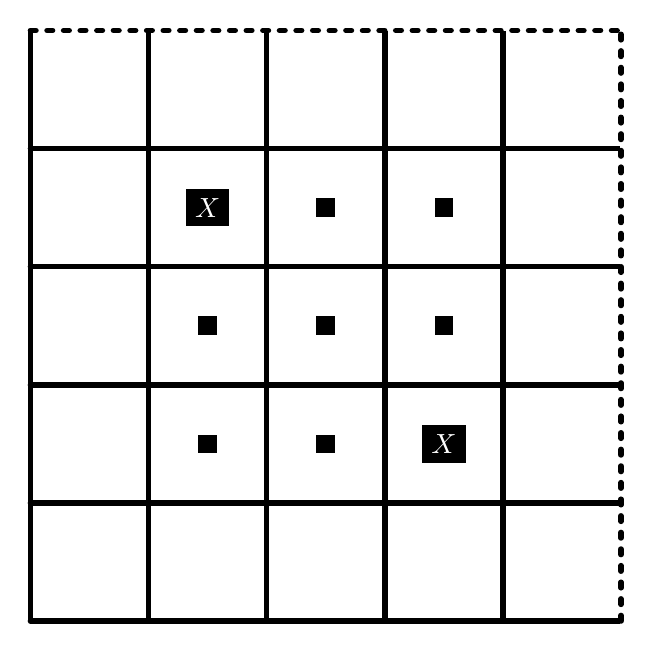
\begin{tikzpicture}[scale=0.75]
\draw[step=2, line width = 2pt, loosely dotted, line cap=round, line join=round] (0,0) grid (10,10);
\draw[step=2, line width = 2pt] (0,0) grid (9.99,9.99);
\foreach \x in {3, 5, 7}{
\foreach \y in {3, 5, 7}{
\node[fill=black] at (\x,\y){};
}
}
\foreach \x/\y/\synd in {3/7/$X$, 7/3/$X$}{
\node[fill=black] at (\x,\y){\textcolor{white}{\synd}};
}

\end{tikzpicture}
\caption{Possible $X$ syndrome pair. 
If the decoder determines that a length-4 chain exists between the two, such a path can be restricted to a bounding box whose interior is marked with black squares above. 
Only if the two syndromes are collinear is there a unique path.}
\end{figure}
\end{itemize}
We'd prefer to have a solution that can handle $Y$ errors `out of the box', to try to put them on the same footing as $X$ and $Z$. 
In the rest of this document, I loosely explore this kind of thing. 
\section{Weights}
To derive the bilinear program, let's first show how the linear program for decoding syndromes independently is derived (see \cite{DKLP} for a longer and stronger explanation).
We begin by writing the probability of an $X$ error that produces pairs of $X$ syndromes, according to an independent error model:
\begin{equation}
p(E_X) = \prod_{C_X \in E_X } p^{\abs{C_X}} (1-p)^{n-\abs{C_X}},
\end{equation}
where $E_X$ is the $X$ error, $C_X$ is a continuous chain of $X$s that makes up part of the error, and $n$ is the number of qubits.
We can simplify this by taking the log: 
\begin{flalign}
p(E_X) &= (1-p)^n \prod_{C_X \in E_X } \left(\frac{p}{1-p} \right)^{\abs{C_X}}\\
& \propto \sum_{C_X \in E_X} \log \left(\frac{p}{1-p} \right)\abs{C_X} \propto -\sum_{C_X \in E_X} \abs{C_X} 
\end{flalign}
Maximizing the likelihood, then, is equivalent to minimizing the sum of lengths of the chains $C_X$ whose endpoints are given by the $X$ (or equivalently $Z$) syndromes. 

We can immediately see the problem. 
A single $Y$ error has an effective weight of two, since it is detected as a length-one $X$ chain and a length-one $Z$ chain in the absence of other errors. 
To fix this, let's make the unjustified assumption that $p_X=p_Y=p_Z$. 
They're going to be different, later (we'll actually have a very different error model later), but this is an easy place to start. 

This results in ``free edges'', since adding a $Z$ error to an edge where there's already an $X$ error results in a $Y$ error, incurring no additional cost. 
\section{Optimisation Problem}
\bibliographystyle{plain}
\bibliography{BilinearProgramForSCDecoding}
\section*{Appendices}
\appendix
\section{Measuring a Different Code Every Round}
If a bilinear program-based decoder doesn't work for whatever reason, do we have the option to measure a different set of stabilisers at every round that commute with the previous round's (e.g. CSS codes with $Y$ and $X$ strings instead of $X$ and $Z$) and reconstruct the error history from there?
A program of research suggests itself, where we go back to DKLP and figure out which errors form chains in 3D given the cycle of stabilisers that we measure. 
\end{document}